\subsection{Quarto sprint}

\begin{minipage}{\textwidth}
  Di seguito è riportata la distribuzione delle ore per ciascun membro del team, accumulate in totali per persona e per ruolo:
  \begin{table}[H]
    \begin{tabularx}{\textwidth}{|c|*{6}{>{\centering}X|}c|}
      \hline
      \multicolumn{8}{|c|}{\textbf{Consuntivo orario}} \\
      \hline
      \textbf{Membro del team} & \textbf{Re} & \textbf{Am} & \textbf{An} & \textbf{Pt} & \textbf{Pr} & \textbf{Ve} & \textbf{Totale per persona} \\
      \hline
      Riccardo Cavalli & 0 & 0 & 0 & 0 & 3 & 5 & 8 \\ 
      \hline
      Raul Pianon & 0 & 0 & 7 & 0 & 0 & 1 & 8 \\ 
      \hline
      Martina Dall'Amico & 0 & 0 & 0 & 6 & 1 & 0 & 7 \\ 
      \hline
      Marco Cristo & 6 & 0 & 0 & 0 & 0 & 2 & 8 \\ 
      \hline
      Sebastiano Lewental & 0 & 6 & 0 & 0 & 0 & 1 & 7 \\ 
      \hline
      Mattia Zecchinato & 0 & 0 & 0 & 3 & 3 & 0 & 6 \\ 
      \hline
      Tommaso Stocco & 0 & 0 & 0 & 0 & 7 & 0 & 7 \\ 
      \hline
      \textbf{Totale ore per ruolo} & 6 & 6 & 7 & 9 & 14 & 9 & \textbf{51} \\
      \hline
    \end{tabularx}
    \caption{Sprint 4 - Consuntivo orario}
  \end{table}
  \end{minipage}
  
  \begin{figure}[H]
    \centering
    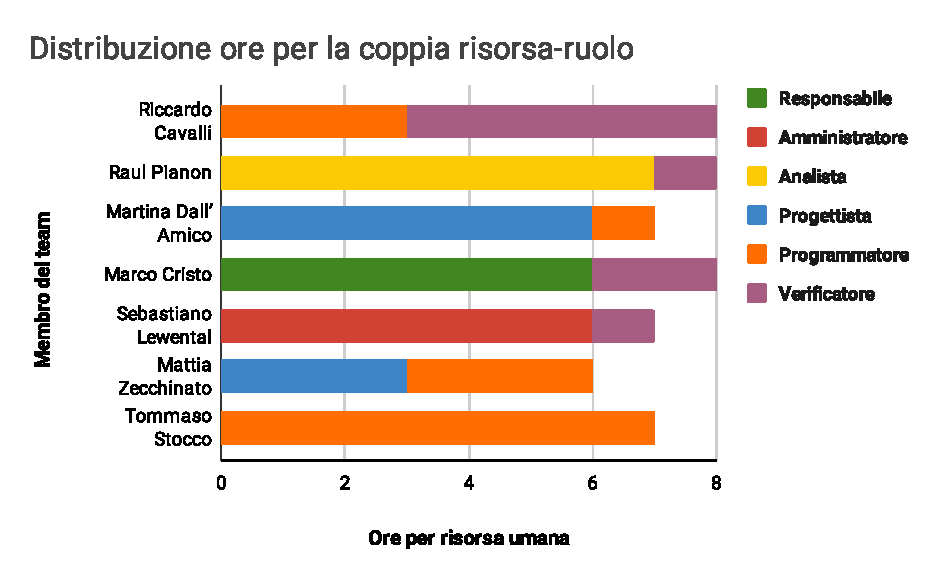
\includegraphics[width=0.90\textwidth]{assets/Consuntivo/Sprint-4/distribuzione_ore_risorsa_ruolo.pdf}
    \caption{Sprint 4 - Istogramma della distribuzione oraria per la coppia risorsa-ruolo}
  \end{figure}
  
  \begin{figure}[H]
    \centering
    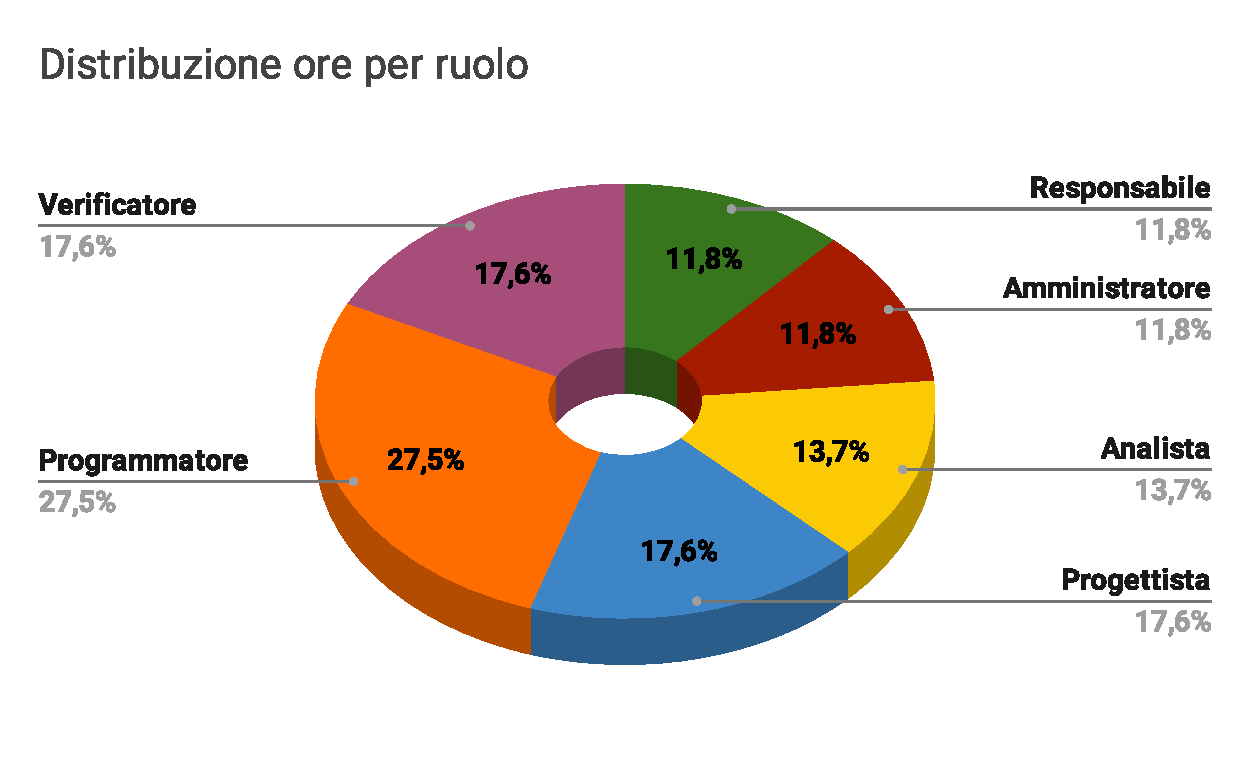
\includegraphics[width=0.90\textwidth]{assets/Consuntivo/Sprint-4/distribuzione_ore_ruolo.pdf}
    \caption{Sprint 4 - Areogramma della distribuzione oraria per ruolo}
  \end{figure}
  
  \begin{minipage}{\textwidth}
  Di seguito è riportato il consuntivo economico del quarto \glossario{sprint}:
  \begin{table}[H]
  \begin{adjustwidth}{-0.5cm}{-0.5cm}
    \centering
    \begin{tabular}{|P{2.9cm}|P{2.3cm}|P{2.5cm}|P{2.3cm}|>{\arraybackslash}P{2.5cm}|}
      \hline
      \multicolumn{5}{|c|}{\textbf{Consuntivo economico}} \\
      \hline
      \textbf{Ruolo} & \textbf{Ore per ruolo} & \textbf{Delta ore preventivo - consuntivo} & \textbf{Costo (in \texteuro)} & \textbf{Delta costo preventivo - consuntivo (in \texteuro)} \\
      \hline
      \Responsabile[U]{} & 6 & 0 & 180,00 & 0,00 \\ \hline
      \Amministratore[U]{} & 6 & 4 & 120,00 & 80,00 \\ \hline
      \Analista[U]{} & 7 & -1 & 175,00 & -25,00 \\ \hline
      \Progettista[U]{} & 9 & 0 & 225,00 & 0,00 \\ \hline
      \Programmatore[U]{} & 14 & -1 & 210,00 & -15,00 \\ \hline
      \Verificatore[U]{} & 9 & 1 & 135,00 & 15,00 \\ \hline
      \textbf{Totale} & \textbf{51} & 3 & \textbf{1.045,00} & 55,00 \\ \hline
      \textbf{Restante} & 446 & / & 8.745,00 & / \\ \hline
      \textbf{Sprint pregressi} & 149 & / & 3.230,00 & / \\ \hline
    \end{tabular}
    \caption{Sprint 4 - Consuntivo economico}
  \end{adjustwidth}
  \end{table}
  \end{minipage}
  
  \begin{figure}[H]
    \centering
    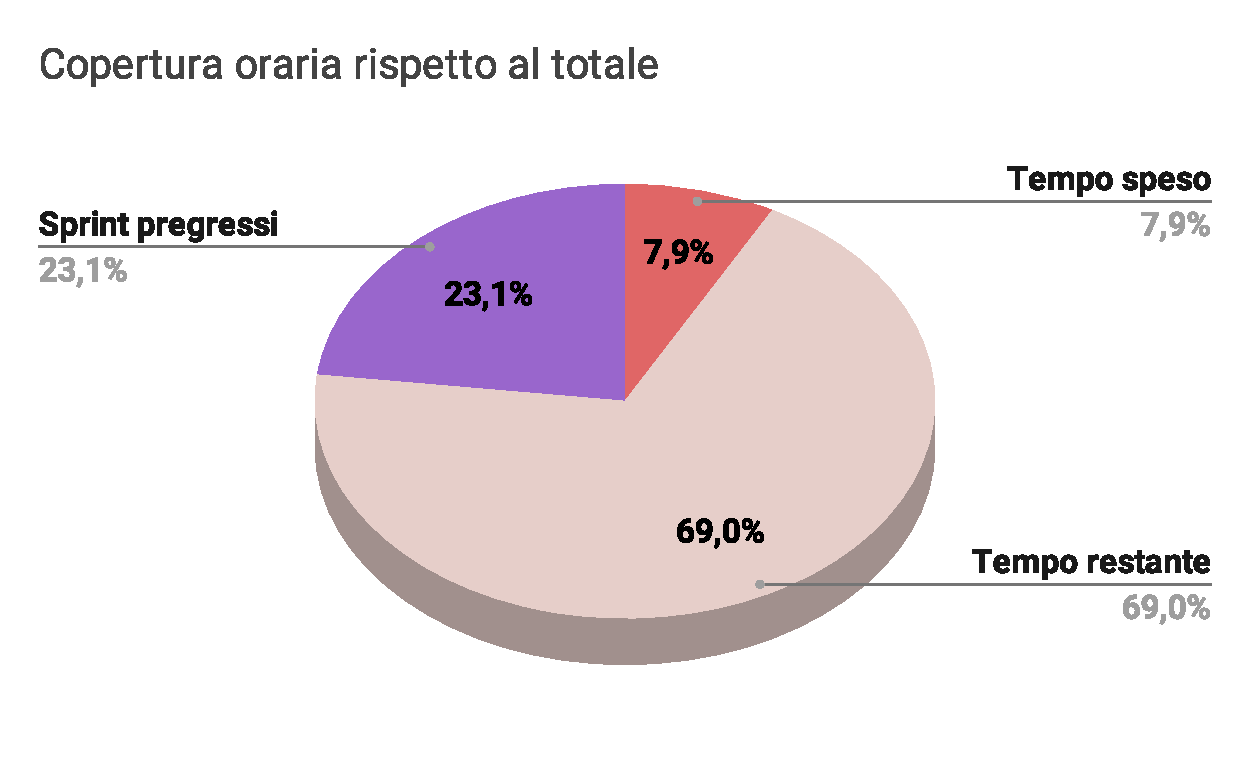
\includegraphics[width=0.90\textwidth]{assets/Consuntivo/Sprint-4/copertura_oraria.pdf}
    \caption{Sprint 4 - Areogramma del tempo speso (in ore) rispetto al totale}
  \end{figure}
  
  \begin{figure}[H]
    \centering
    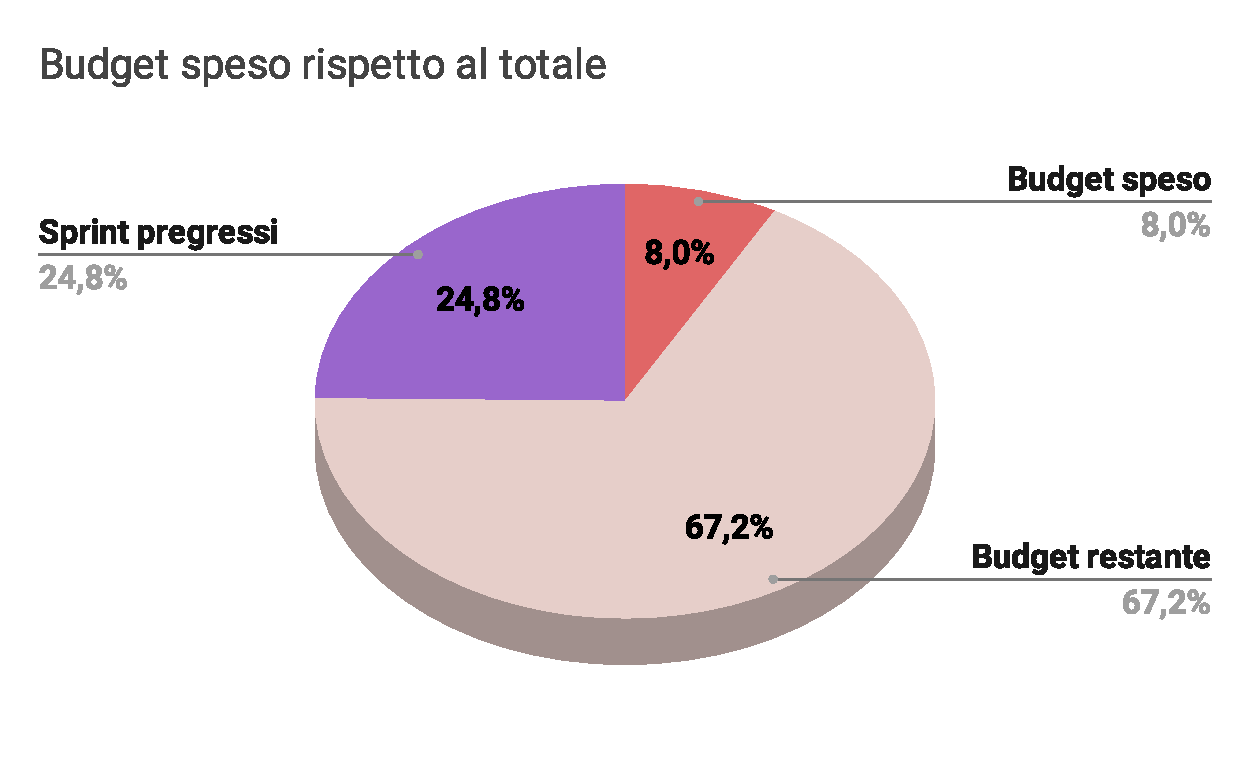
\includegraphics[width=0.90\textwidth]{assets/Consuntivo/Sprint-4/budget_speso.pdf}
    \caption{Sprint 4 - Areogramma del budget speso rispetto al totale}
  \end{figure}
  
  \begin{minipage}{\textwidth}
    Di seguito sono riportate le ore rimanenti per la coppia risorsa-ruolo:
    \begin{table}[H]
      \begin{tabularx}{\textwidth}{|c|*{6}{>{\centering}X|}c|}
        \hline
        \multicolumn{8}{|c|}{\textbf{Ore rimanenti per la coppia risorsa-ruolo}} \\
        \hline
        \textbf{Membro del team} & \textbf{Re} & \textbf{Am} & \textbf{An} & \textbf{Pt} & \textbf{Pr} & \textbf{Ve} & \textbf{Totale per persona} \\
        \hline
        Riccardo Cavalli & 0 & 2 & 9 & 14 & 18 & 16 & 59 \\ 
        \hline
        Raul Pianon & 2 & 10 & 2 & 20 & 15 & 12 & 61 \\ 
        \hline
        Martina Dall'Amico & 9 & 2 & 1 & 14 & 22 & 16 & 64 \\ 
        \hline
        Marco Cristo & 3 & 10 & 2 & 17 & 13 & 17 & 62 \\ 
        \hline
        Sebastiano Lewental & 9 & 4 & 2 & 11 & 21 & 17 & 64 \\ 
        \hline
        Mattia Zecchinato & 9 & 9 & 3 & 11 & 20 & 15 & 67 \\ 
        \hline
        Tommaso Stocco & 5 & 4 & 3 & 20 & 16 & 19 & 67 \\ 
        \hline
        \textbf{Totale ore per ruolo} & 37 & 42 & 22 & 107 & 126 & 112 & \textbf{446} \\ 
        \hline
      \end{tabularx}
      \caption{Sprint 4 - Ore rimanenti per la coppia risorsa-ruolo}
    \end{table}
  \end{minipage}

\subsubsection{Revisione delle attività}

Nell'arco del quarto \glossario{sprint}, il team ha svolto le seguenti attività:
\begin{itemize}
    \item Stesura verbali interni ed esterni;
    \item Revisione dei consuntivi pregressi all'interno del \PdP;
    \item Rielaborazione completa dei \glossario{casi d'uso} nell'\AdR;
    \item Estensione dei casi d'uso nell'\AdR\ in accordo con il team di programmatori;
    \item Creazione e connessione al database;
    \item Sviluppo dell'interfaccia di login tramite \glossario{Streamlit};
    \item \glossario{Dockerizzazione} dell'ambiente di sviluppo;
    \item Definizione dei test di correttezza del \glossario{prompt};
    \item Scelta definitiva del modello \glossario{LLM};
    \item Creazione della lista di selezione del dizionario dati;
    \item Sviluppo back-end della funzionalità di debug per il profilo Tecnico;
    \item Riorganizzazione del repository ChatSQL per integrare i moduli e rimuovere i file ridondanti;
    \item Refactoring completo del codice con rimozione dei file obsoleti.
\end{itemize}

\subsubsection{Retrospettiva}

\par Di seguito sono riportati i risultati del questionario di valutazione dello \glossario{sprint}:
\begin{itemize}
  \item Organizzazione dello \glossario{sprint}\ - Valutazione: 7;
  \item Conduzione dei meeting interni - Valutazione: 8;
  \item Conduzione dei meeting esterni - Valutazione: 8;
  \item Impegno e partecipazione dei singoli membri - Valutazione: 9;
  \item La quasi totalità dei membri del team era a conoscenza delle proprie mansioni;
  \item La numerosità delle riunioni è risultata adeguata per circa la metà dei membri; inoltre, il team preferirebbe organizzare più incontri informali tra programmatori;
  \item Le riunioni sono state organizzate quasi sempre con il giusto preavviso;
  \item Il rapporto ore spese/ore produttive è risultato meno equilibrato rispetto allo \glossario{sprint} precedente;
  \item La produttività generale ha raggiunto una buona soglia;
  \item Alcuni membri del team ritengono opportuno avere maggiori dettagli sulle task a medio/lungo termine.
\end{itemize}

\vspace{0.5\baselineskip}
\par A seguire le \textbf{analisi a posteriori} del quarto \glossario{sprint}:
\begin{itemize}
  \item La sola pianificazione delle attività, per quanto dettagliata, non ha consentito a tutti i membri del team di prendere in carico le proprie task a inizio \glossario{sprint}. Alcuni componenti del gruppo, infatti, hanno incontrato difficoltà nel mantenere l'allineamento con la mole di lavoro elaborata negli sprint precedenti, specialmente riguardo alla coerenza dei contenuti. Per tale motivo il flusso di lavoro ha subito qualche giorno di rallentamento;
  \item Il gruppo ha stabilito che, a partire dal prossimo sprint, ciascun componente dovrà documentare, o spiegare tramite riunioni ad hoc, il lavoro pianificato per i ruoli entranti;
  \item Come conseguenza del punto precedente, il team ha deciso di affiancare al \Responsabile{}, per l'assegnazione delle task, i membri che hanno già ricoperto un determinato ruolo. In questo modo, il gruppo ritiene di poter delineare con maggior puntualità le attività imminenti;
  \item Anche se i risultati del questionario hanno evidenziato una sufficiente adeguatezza organizzativa riguardo le riunioni, il \Responsabile{} ha ritenuto opportuno aumentare il margine di preavviso. L'obiettivo è minimizzare le assenze durante i meeting, comunicando il calendario delle riunioni future entro la fine dello sprint;
  \item Nonostante il team abbia organizzato una quantità apprezzabile di incontri tra programmatori e altri ruoli correlati durante la seconda metà dello sprint, lo stesso non si può dire per la prima settimana. Ciò ha portato a dei ritardi nella prosecuzione delle attività, mantenendo comunque alto l'impegno individuale e, di conseguenza, inficiando sul rapporto tra le ore spese e quelle produttive. Preso atto di ciò, il gruppo ha prontamente affrontato il problema e ha incrementato il numero di riunioni, recuperando così lo stallo iniziale.
\end{itemize}

\subsubsection{Aggiornamento pianificazione e preventivo}
\par Il team ha definito un piano d'azione per migliorare l'organizzazione e la produttività del prossimo \glossario{sprint}:
\begin{itemize}
  \item Aumentare il preavviso per i meeting futuri;
  \item I ruoli uscenti devono affiancare, ove possibile, il \Responsabile{} nella definizione delle task per i ruoli entranti;
  \item Incrementare il numero di riunioni informali tra membri che ricoprono ruoli analoghi;
  \item Effettuare una separazione più netta tra \glossario{front-end} e \glossario{back-end}.
\end{itemize}

\paragraph*{Pianificazione futura:}
\par Con l'avvicinarsi della scadenza per la \RTB, il focus della pianificazione si sposterà sull'integrazione tra front-end e back-end utilizzando le tecnologie approfondite dal team nello sprint appena concluso. In parallelo, sarà fondamentale verificare e rivedere i documenti, con un'attenzione particolare al \PdP per aggiornare il preventivo a finire dello sprint 4 e redistribuire le ore per ruolo. Un incontro con il Professore Riccardo Cardin è stato programmato per chiarire eventuali dubbi sulle tecnologie scelte.
Nello specifico, le attività tecniche previste comprendono la configurazione di Flask e Vue.js, la connessione al database, e la gestione CRUD del dizionario dati in backend. Si procederà anche con la progettazione della struttura generale del front-end, nonché con la visualizzazione dei log e del dizionario dati lato front-end. Inoltre, saranno svolti ulteriori approfondimenti sul funzionamento di txtai.
Per quanto riguarda la documentazione, oltre alla revisione del \PdP, il team si impegnerà nella stesura e verifica dei verbali interni ed esterni, e nell'ampliamento dei casi d'uso nell'\AdR, includendo estensioni ed errori e integrando i grafici dei casi d'uso rimanenti.

\paragraph*{Preventivo "a finire" (\sezione{sec:stima_temporale}):}
\par Data la numerosità delle risorse assegnate originariamente al ruolo di \Progettista{}, il team ha concordato la necessità di ridistribuire tali risorse a favore dell'\Amministratore{}, il cui impegno orario è stato ritenuto sottostimato. Questa ripartizione ha portato a un lieve aumento delle ore produttive totali per i ruoli di \Programmatore{} e di \Verificatore{}. 
La ripartizione è avvenuta come segue:
\begin{itemize}
  \item Le ore complessive assegnate al ruolo di \Progettista{} sono diminuite da 161 a 140;
  \item Le ore complessive assegnate al ruolo di \Amministratore{} sono aumentate da 56 a 70;
  \item Le ore complessive assegnate al ruolo di \Programmatore{} sono aumentate da 154 a 161;
  \item Le ore complessive assegnate al ruolo di \Verificatore{} sono aumentate da 140 a 147;
\end{itemize}
Il monte ore individuali è di conseguenza aumentato da 91 a 92.

\paragraph*{Gestione dei rischi (\sezione{sec:analisi_rischi})}
\par Nel corso del quarto \glossario{sprint}, il seguente rischio non è stato gestito con successo:
\begin{itemize}
  \item \textbf{RO4 - Rotazione dei ruoli}: diversi membri del team hanno incontrato degli ostacoli a seguito della rotazione dei ruoli. Una volta individuata tale problematica, dopo una serie di confronti interni, è stata attuata la contromisura descritta nella \sezione{sec:analisi_rischi}. L'efficacia del metodo di mitigazione ha subito però una riduzione a causa della sua applicazione tardiva, causando un periodo di rallentamento iniziale. La gestione del rischio deve quindi essere modificata, per aggiungere ulteriori controlli nelle strategie di rilevamento.
\end{itemize}

\vspace{0.5\baselineskip}
\par Di seguito sono elencati i rischi gestiti con successo:
\begin{itemize}
  \item \textbf{RP1 - Questioni personali}: nel corso dello \glossario{sprint}, un membro del team ha incontrato difficoltà nello svolgimento delle proprie mansioni per motivi personali. La gestione anticipata di questa situazione (mediante comunicazione preventiva) ha consentito al gruppo di ricalibrare e ridistribuire le attività precedentemente assegnate, garantendo che il flusso di lavoro rimanesse stabile;
  \item \textbf{RT1 - Scarso know-how tecnologico}: nonostante le difficoltà nell’approfondimento della libreria \glossario{FAISS}, il team ha formato una squadra di due membri dedicata allo studio della documentazione ufficiale, garantendo così il raggiungimento degli obiettivi prefissati.
  \item \textbf{RT2 - Malfunzionamenti hardware}: i guasti di natura hardware sono stati mitigati attraverso l’integrazione continua delle modifiche nell'ambiente condiviso.
\end{itemize}
